\title{Lecture 13\\Representation of Ontologies in a Knowledge Base}

\begin{frame}
	\titlepage
\end{frame}

\begin{frame}{\\Lecture outline}
	\topline
	\justifying
	The concept of an ontology and the classification of ontologies. Integrated ontologies. How ontologies relate to subject domains and semantic neighborhoods. Representation of ontologies in a knowledge base.
\end{frame}

\begin{frame}{\\The concept of an ontology}
	\topline
	\justifying
	\begin{SCn}
		\scnheader{ontology}
		\scnidtf{formalization of the conceptualization of a subject domain}
		\begin{scnindent}
			\scntext{explanation}{A concept is a notion.}
		\end{scnindent}
		\scnidtf{system of concepts that describe the properties of a subject domain}
		\scniselement{type of knowledge}

		\scnheader{sc-ontology*}
		\scnidtf{specification (formal description) of a subject domain}
		\scnrelfrom{second domain}{ontology}
		\scnrelfrom{first domain}{subject domain}
	\end{SCn}
\end{frame}

\begin{frame}{\\Ontology}
	\topline
	\justifying
	\vspace{5mm}
	\begin{SCn}
		\scnheader{sc-ontology}
		\scnidtf{union of semantic neighborhoods of a specified type that describe the properties of all concepts under study in the given subject domain}
		\begin{figure}[H]
			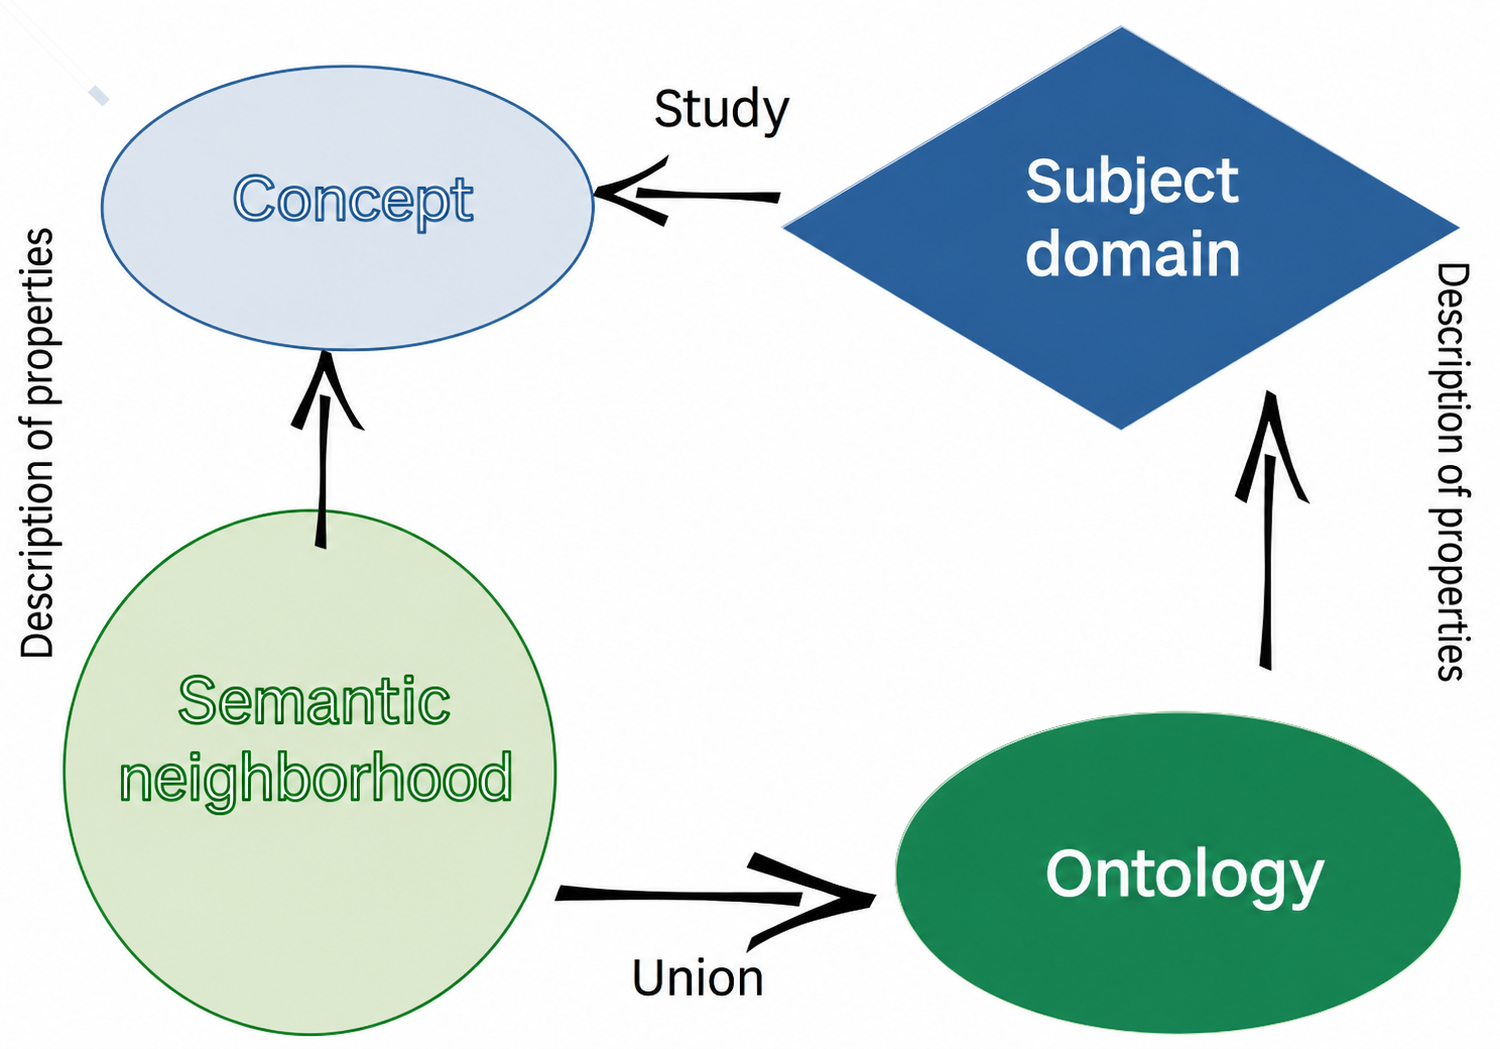
\includegraphics[width=0.62\linewidth,height=0.48\textheight,keepaspectratio]{figures/sd_ontologies/ontology_en.png}
		\end{figure}
	\end{SCn}
\end{frame}

\begin{frame}{\\Classification of ontologies}
	\topline
	\justifying
	\vspace{10mm}
	\begin{SCn}
		\scnheader{sc-ontology}
		\scnsuperset{structural specification}
		\begin{scnindent}
			\begin{scnrelfromset}{concepts used}
				\scnitem{maximal class of objects of study\scnrolesign}
				\scnitem{class of objects of study\scnrolesign}
				\scnitem{child subject domain*}
				\scnitem{related subject domain*}
			\end{scnrelfromset}
		\end{scnindent}
		\scnsuperset{set-theoretic specification}
		\begin{scnindent}
			\begin{scnrelfromset}{concepts used}
				\scnitem{inclusion*}
				\scnitem{partition*}
				\scnitem{properties of relations}
				\scnitem{intersection*}
			\end{scnrelfromset}
		\end{scnindent}
	\end{SCn}
\end{frame}

\begin{frame}{\\Classification of ontologies (continued)}
	\topline
	\justifying
	\vspace{10mm}
	\small
	\begin{SCn}
		\scnheader{sc-ontology}
		\scnsuperset{terminological specification}
		\begin{scnindent}
			\begin{scnrelfromset}{concepts used}
				\scnitem{identifier*}
				\scnitem{identification rules}
			\end{scnrelfromset}
		\end{scnindent}
		\scnsuperset{logical specification}
		\begin{scnindent}
			\begin{scnrelfromset}{concepts used}
				\scnitem{logical proposition}
				\scnitem{theorem\scnrolesign}
				\scnitem{axiom\scnrolesign}
				\scnitem{logical hierarchy of concepts*}
				\begin{scnindent}
					\scnsuperset{concepts used to define the given concept*}
					\scnsuperset{concepts defined in terms of the given concept*}
				\end{scnindent}
			\end{scnrelfromset}
		\end{scnindent}
	\end{SCn}
\end{frame}

\begin{frame}{\\Integrated ontology}
	\topline
	\justifying
	\begin{SCn}
		\scnheader{integrated ontology}
		\scnidtf{union of all types of ontologies for the given subject domain}
	\end{SCn}
\end{frame}

\begin{frame}{\\Ontology example}
	\topline
	\justifying
	\vspace{7mm}
	\begin{figure}[H]
		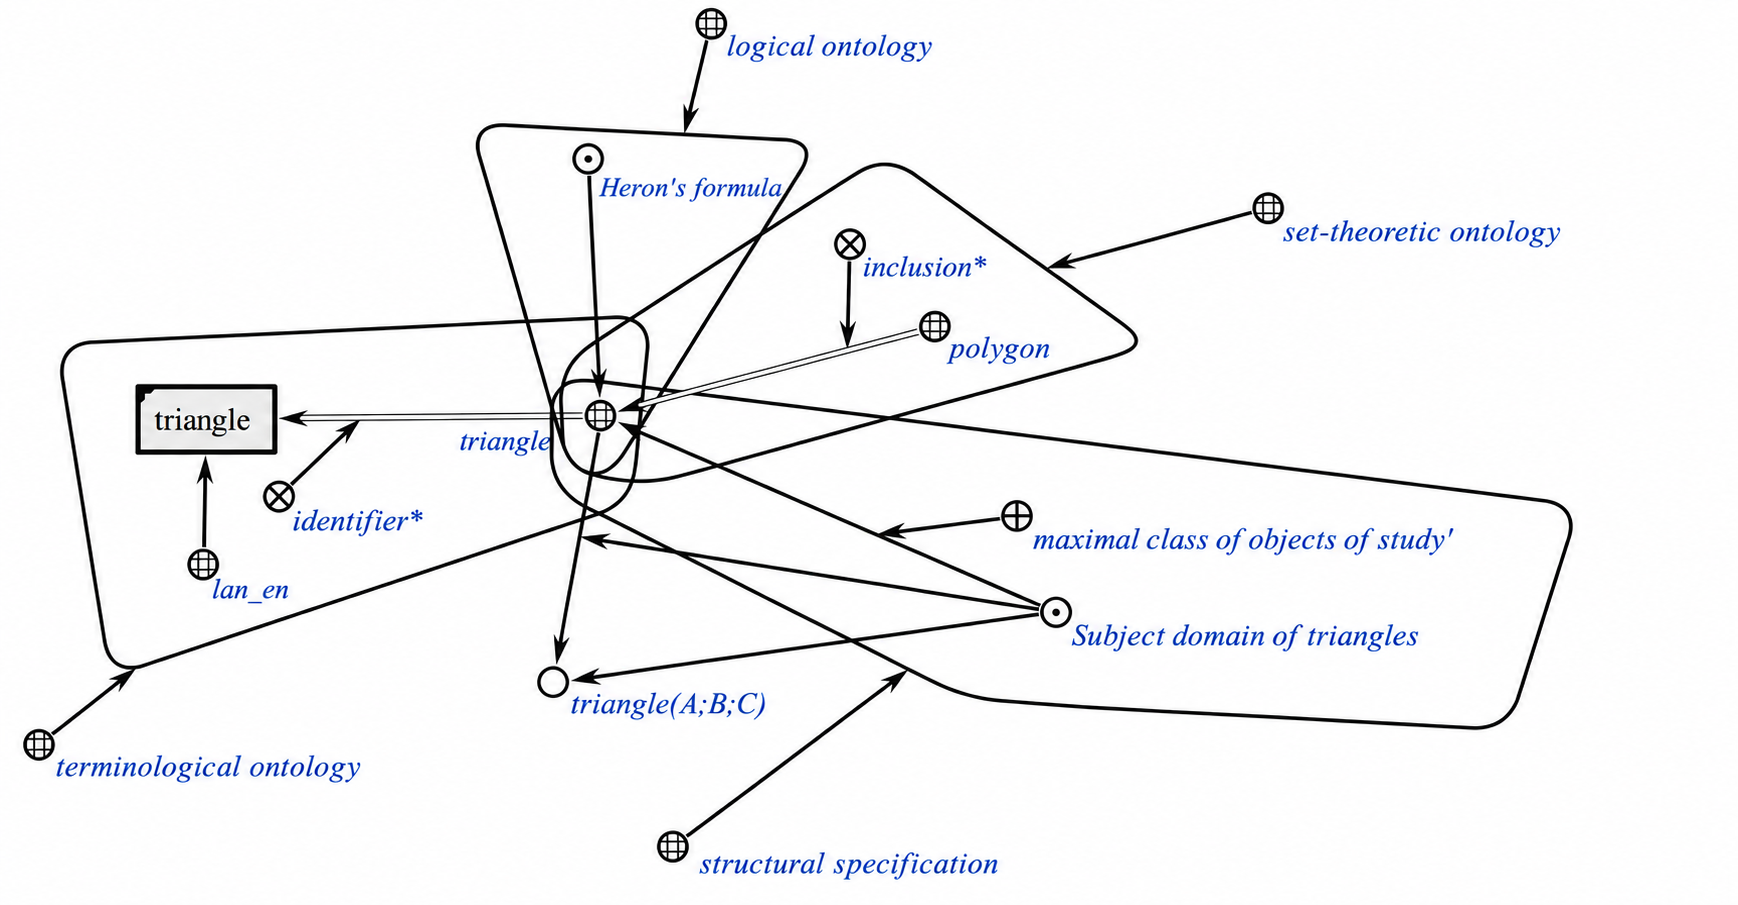
\includegraphics[width=\linewidth,height=0.73\textheight,keepaspectratio]{figures/sd_ontologies/ontology1_en.png}
	\end{figure}
\end{frame}

\begin{frame}{\\Ontology examples}
	\topline
	\justifying
	\vspace{7mm}
	\begin{figure}[H]
		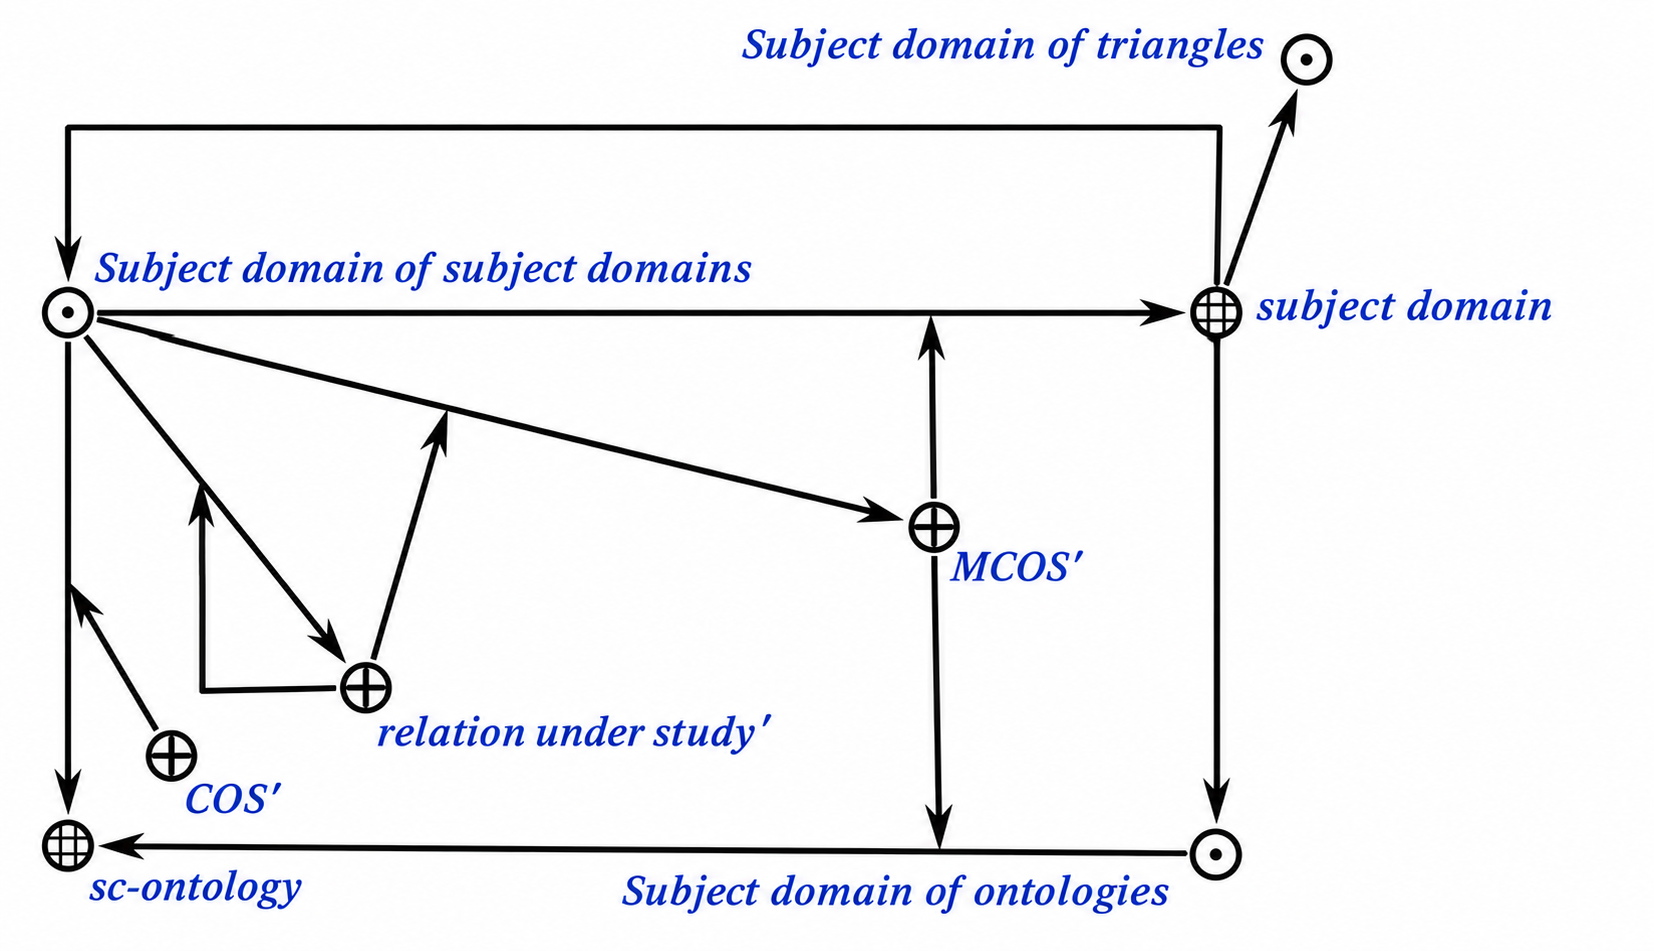
\includegraphics[width=\linewidth,height=0.65\textheight,keepaspectratio]{figures/sd_ontologies/ontology2_en.png}
	\end{figure}
	{\footnotesize \textit{COS}: class of objects of study. \textit{MCOS}: maximal class of objects of study.}
\end{frame}

\begin{frame}{\\Ontology example}
	\topline
	\justifying
	\vspace{7mm}
	\begin{figure}[H]
		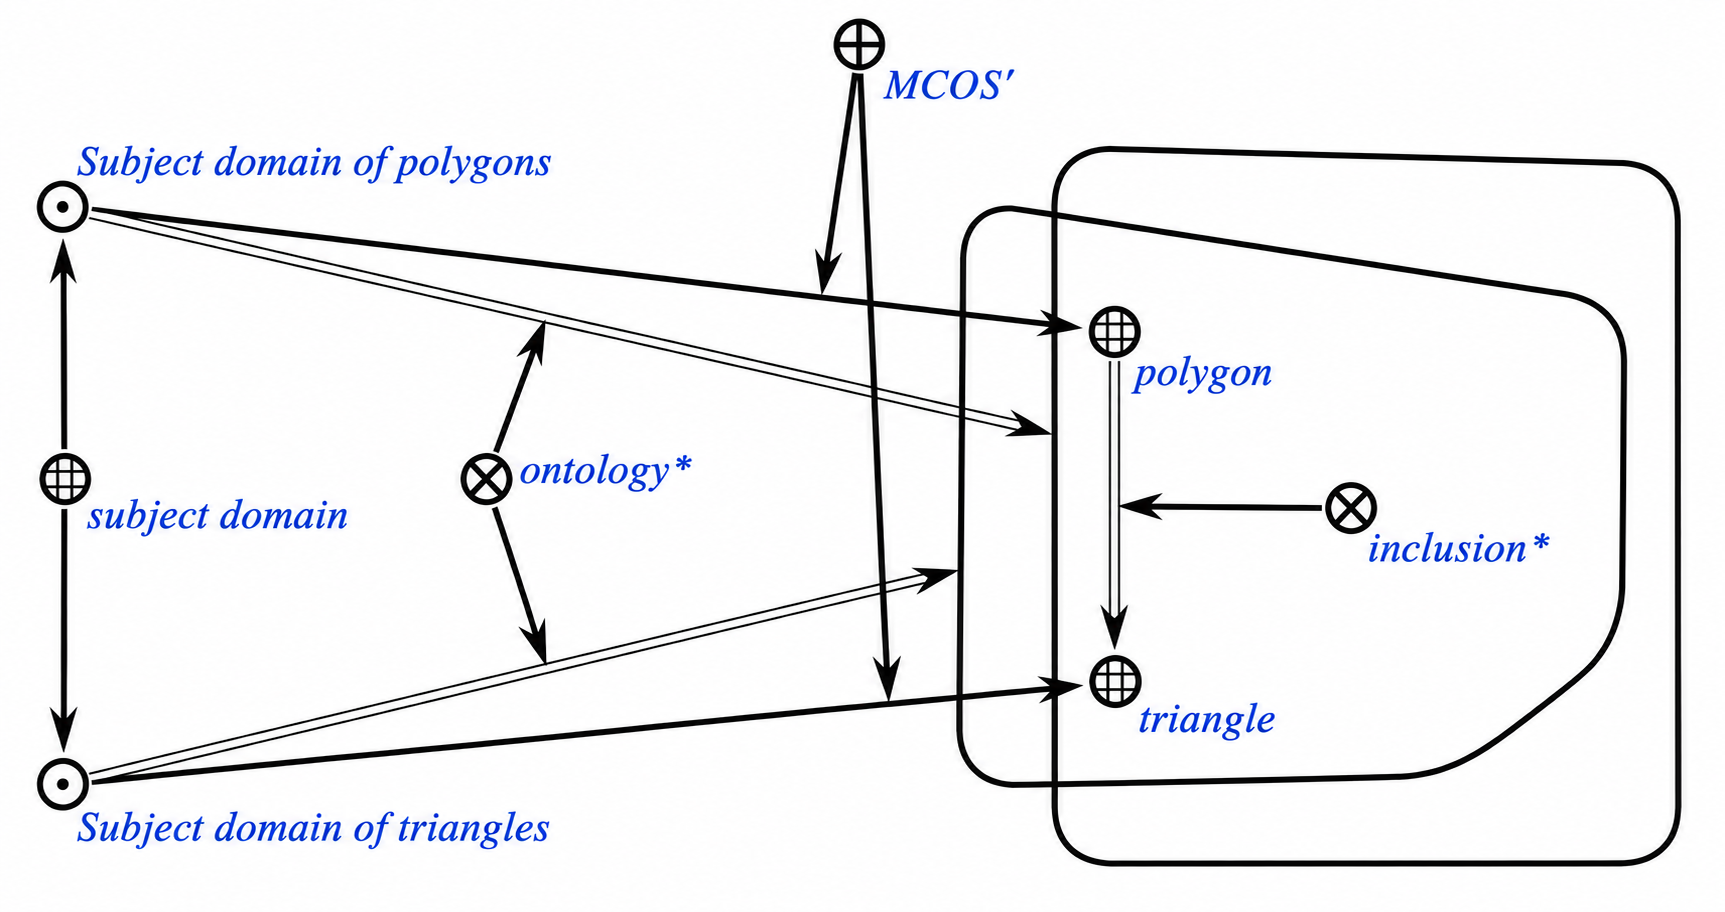
\includegraphics[width=\linewidth,height=0.65\textheight,keepaspectratio]{figures/sd_ontologies/ontology3_en.png}
	\end{figure}
	{\footnotesize \textit{MCOS}: maximal class of objects of study.}
\end{frame}
